\apendice{Especificación de Requisitos}
\section{Introducción}
En este punto se detallan los requisitos con que debe cumplir el proyecto y que determinarán restricciones, funcionalidades y comportamiento de éste. 

\section{Objetivos generales}
Los objetivos generales enmarcan la funcionalidad del proyecto, que se detallan a continuación:
\begin{itemize}
    \item Crear una plataforma que consiga aumentar confort, comodidad y seguridad dentro del domicilio.
    \item Generar un Sistema Domótico que nos permita automatizar parámetros de la vivienda así como poder ordenar acciones en tiempo real.
    \item Crear un Sistema Simulador de Presencia Domiciliaria de funcionamiento autónomo.
    \item Debe contar con una interfaz de comunicación multiplataforma para interactuar con el software.
\end{itemize}

\section{Catálogo de requisitos}
En este punto se desglosan los requisitos con que debe cumplir el proyecto, derivando de los anteriormente expuestos.

\subsection{\textbf{Requisitos funcionales}}

\begin{itemize}
    \item \textbf{RF-1 Obtención de datos:} El Sistema debe ser capaz de obtener datos necesarios para su correcto funcionamiento.
    \begin{itemize}
        \item \textbf{RF-1.1 Obtención de ubicación:} Debe ser capaz de determinar su ubicación geográfica.
        \item \textbf{RF-1.2 Obtención de posición solar:} Debe poder obtener información sobre la posición solar con respecto del planeta según su ubicación geográfica.
        \item \textbf{RF-1.3 Obtención de temperaturas:} Debe poder obtener información meteorológica de las próximas horas en la ubicación en la que se encuentra el Sistema.
        \item \textbf{RF-1.4 Datos bajo demanda:} El usuario debe poder solicitar la obtención de los datos bajo demanda.
    \end{itemize}

    \item \textbf{RF-2 Control de periféricos:} El Sistema debe poder controlar los periféricos que tiene conectados.
    \begin{itemize}
        \item \textbf{RF-2.1 Control automático:} El sistema debe poder controlar de forma autónoma los dispositivos conectados.
        \item \textbf{RF-2.2 Control instantáneo:} El usuario debe poder controlar los diferentes periféricos a placer.
        \item \textbf{RF-2.3 Control planificado:} El sistema debe poder planificar el control de los periféricos conectados.
        \item \textbf{RF-2.4 Parametrización:} El usuario debe poder parametrizar la automatización de los periféricos.
    \end{itemize}
    
    \item \textbf{RF-3 Información:} La información de que dispone el sistema siempre estará a disposición del usuario.
    \begin{itemize}
        \item \textbf{RF-3.1 Información de sistema:} El usuario podrá obtener información básica sobre el sistema.
        \item \textbf{RF-3.2. Información de planificación:} El usuario debe poder obtener información sobre la planificación de la automatización de los periféricos.
        \item \textbf{RF-3.3. Información parametrización:} El usuario debe poder obtener información sobre la parametrización de la automatización de los periféricos.
        \item \textbf{RF-3.4 Diagramas:} El usuario debe poder obtener un diagrama de temperaturas del día u otros días anteriores que estén archivados en la máquina a modo de registro.
    \end{itemize}
    
    \item \textbf{RF-4 Control máquina:} Se deben poder ejecutar algunas tareas básicas sobre la máquina que soporta el Sistema.
    \begin{itemize}
        \item \textbf{RF-4.1 Operaciones bajo demanda:} El usuario podrá apagar y reiniciar la máquina siempre que lo desee.
        \item \textbf{RF-4.2 Operaciones automáticas:} El sistema se reiniciará, al menos, una vez al día.
    \end{itemize}   
    
    \item \textbf{RF-5 Gestión de la máquina:} La máquina que soporta el sistema debe poder ser accesible por parte del usuario.
    \begin{itemize}
        \item \textbf{RF-5.1 Gestión local:} El usuario podrá gestionar el sistema Operativo de la máquina que soporta el Sistema de forma local.
        \item \textbf{RF-5.2 Gestión remota:} El usuario podrá gestionar el sistema Operativo de la máquina que soporta el Sistema de forma remota vía VNC.
    \end{itemize}
    
    \item \textbf{RF-6 Comunicación entre BackEnd y FrontEnd:} Debe existir un filtro en las comunicaciones.
    \begin{itemize}
        \item \textbf{RF-6.1 Selección de usuarios:} El propio usuario debe poder gestionar los usuarios que pueden interactuar con el Sistema.
        \item \textbf{RF-6.2 Rechazo de peticiones:} Los usuarios que no estén admitidos en la lista no podrán acceder a la comunicación con el Sistema.
        \item \textbf{RF-6.3 Interacción multiplataforma:} Debe poder interactuar mediante las aplicaciones móviles existentes de Telegram y desde cualquier navegador popularmente extendido como pueden ser Chrome, Edge o Firefox entre otros. 
    \end{itemize}
\end{itemize}

\subsection{\textbf{Requisitos no funcionales}}

\begin{itemize}
    \item \textbf{RNF-1 Escalabilidad:} Debe poder ampliarse fácilmente.
    \item \textbf{RNF-2 Eficiencia:} Debe minimizar la carga computacional para minimizar también el consumo energético del Sistema, además de permitir que la temperatura exterior incida en menos medida en las condiciones deseadas optimizando el consumo de recursos.
    \item \textbf{RNF-3 Rendimiento:} El sistema debe ser fluido y evitar cargas innecesarias.
    \item \textbf{RNF-4 Usabilidad:} El FrontEnd debe ser lo más usable posible, es decir, fácil de utilizar y aprender e intuitivo, y adaptado a las necesidades que pretende cubrir.
    \item \textbf{RNF-5 Disponibilidad:} El Sistema debe estar siempre en correcto funcionamiento.
    \item \textbf{RNF-6 Durabilidad:} El software debe poder funcionar correctamente durante un tiempo relativamente largo.
    \item \textbf{RNF-7 Capacidad:} Debe poder obtener la información necesaria y actuar conforme a lo que se espera de él.
    \item \textbf{RNF-8 Documentación:} Debe existir la suficiente documentación para poder implementar e interactuar con el Sistema.
    \item \textbf{RNF-9 Operabilidad:} Debe permitir manejar y controlar el Sistema según los requisitos funcionales.
    \item \textbf{RNF-10 Mantenibilidad:} Debe desarrollarse de tal manera que el mantenimiento sea lo más fácil y rápido posible.
    \item \textbf{RNF-11 Seguridad:} Todas las operaciones desde el FrontEnd deben ser seguras y estar cifradas.
    \item \textbf{RNF-12 Legibilidad:} El software debe ser fácilmente legible.
    \item \textbf{RNF-13 Extensibilidad:} El código debe ser fácilmente adaptable y reutilizable.
    \item \textbf{RNF-14 Liberación de código:} Debe disponer de un Sistema Operativo GNU y el código debe tener algún tipo de licencia GNU.
    \item \textbf{RNF-15 Respaldo documental:} Toda la instalación debe realizarse conforme a los estándares legales vigentes.
~\\~\\~\\~\\
\end{itemize}

\section{Especificación de requisitos}
La especificación de requisitos contempla los casos de uso contra nuestro código.
Además, también podemos ver el diagrama de los casos de uso, aunque lo he dividido en los diagramas <<1/2>>~\ref{CDU1} y <<2/2>>~\ref{CDU2}

\begin{figure}[h]
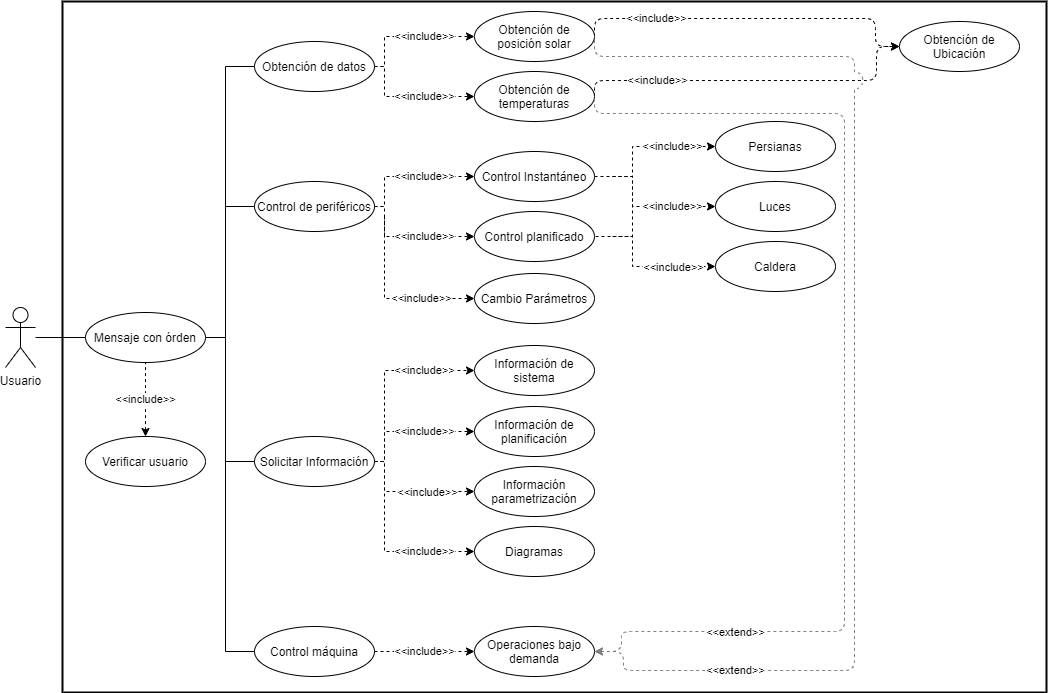
\includegraphics[width=1.15\textwidth]{img/Diagramas/CasosDeUso.png}
\caption{Casos de uso 1/2.}\label{CDU1}
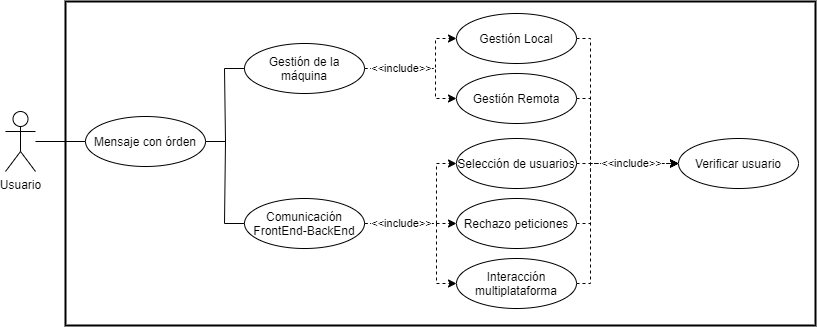
\includegraphics[width=0.85\textwidth]{img/Diagramas/CasosDeUsoBackEnd.png}
\caption{Casos de uso 2/2.}\label{CDU2}
\end{figure}

\subsection{Actores}
Los actores serán cada uno de los usuarios del Sistema que controlará el sistema desde el FrontEnd.

\footnotesize%%%%%%%%%%%  smaller font size %%%%%%%%
\begin{longtable}{>{\hspace{0pt}}m{0.182\linewidth}>{\hspace{0pt}}m{0.758\linewidth}}
\hline
\rowcolor[rgb]{0.937,0.937,0.937} \multicolumn{1}{|>{\hspace{0pt}}m{0.182\linewidth}|}{\textbf{CU-01}} & \multicolumn{1}{>{\hspace{0pt}}m{0.758\linewidth}|}{\textbf{Obtención de posición solar}} \endfirsthead 
\hline
\textbf{Versión} & 1.0 \\
\rowcolor[rgb]{0.937,0.937,0.937} \textbf{Actor} & Usuario \\
\textbf{Requisitos asociados} & RF-1, RF-1.1, RF-1.2, RF-1.3, RF-1.4 \\
\rowcolor[rgb]{0.937,0.937,0.937} \textbf{Descripción} & Permite al usuario obtener los datos necesarios para parametrizar el Sistema Domótico Inteligente. \\
\textbf{Precondición} & \begin{tabular}{@{\labelitemi\hspace{\dimexpr\labelsep+0.5\tabcolsep}}l}Al ser un proceso principalmente automático, únicamente se~\end{tabular}\par{}~ ~ requiere una línea de datos con acceso a Internet.\par\par{}\begin{tabular}{@{\labelitemi\hspace{\dimexpr\labelsep+0.5\tabcolsep}}l}En el caso de hacer la petición el usuario, también necesita~\end{tabular}\par{}~ ~ ser uno de los usuarios autorizados. \\
\rowcolor[rgb]{0.937,0.937,0.937} \textbf{Acciones} & \begin{tabular}{@{\labelitemi\hspace{\dimexpr\labelsep+0.5\tabcolsep}}>{\cellcolor[rgb]{0.937,0.937,0.937}}l}El usuario solicita la obtención inmediata de los datos~\end{tabular}\par{}necesarios para realizar la próxima programación.\par\par{}\begin{tabular}{@{\labelitemi\hspace{\dimexpr\labelsep+0.5\tabcolsep}}>{\cellcolor[rgb]{0.937,0.937,0.937}}l}El programa llama a las APIS de geolocalización,~\end{tabular}\par{}astrológicos y meteorológicos. \\
\textbf{Postcondición} & El bot lanza los scripts de recopilación de datos y almacena los datos. \\
\rowcolor[rgb]{0.937,0.937,0.937} \textbf{Excepciones} & Si no puede recopilar los datos envía mensaje al usuario. \\
\textbf{Importancia} & Alta \\\hline\\
\caption{CU-01 - Obtención de datos}\\ 
\end{longtable}


\begin{longtable}{>{\hspace{0pt}}m{0.278\linewidth}>{\hspace{0pt}}m{0.662\linewidth}}
\hline
\rowcolor[rgb]{0.937,0.937,0.937} \multicolumn{1}{|>{\hspace{0pt}}m{0.278\linewidth}|}{\textbf{CU-02}} & \multicolumn{1}{>{\hspace{0pt}}m{0.662\linewidth}|}{\textbf{Control de periféricos}} \endfirsthead 
\hline
\textbf{Versión} & 1.0 \\
\rowcolor[rgb]{0.937,0.937,0.937} \textbf{Actor} & Usuario \\
\textbf{Requisitos asociados} & RF-2, RF-2.1, RF-2.2, RF-2.3, RF-2.4 \\
\rowcolor[rgb]{0.937,0.937,0.937} \textbf{Descripción} & Permite controlar los periféricos \\
\textbf{Precondición} & \begin{tabular}{@{\labelitemi\hspace{\dimexpr\labelsep+0.5\tabcolsep}}l}Deben existir periféricos y estar configurados en el~\end{tabular}\par{}archivo al efecto.\par\par{}\begin{tabular}{@{\labelitemi\hspace{\dimexpr\labelsep+0.5\tabcolsep}}l}El usuario debe estar acreditado.\end{tabular} \\
\rowcolor[rgb]{0.937,0.937,0.937} \textbf{Acciones} & \begin{tabular}{@{\labelitemi\hspace{\dimexpr\labelsep+0.5\tabcolsep}}>{\cellcolor[rgb]{0.937,0.937,0.937}}l}El usuario puede ordenar controlar un elemento.\end{tabular} \\
\textbf{Postcondición} & El~periférico cambia de estado. \\
\rowcolor[rgb]{0.937,0.937,0.937} \textbf{Excepciones} & Si no puede realizar la acción envía mensaje al usuario. \\
\textbf{Importancia} & Media \\
\hline\\
\caption{CU-02 - Control de periféricos.}~\\~\\~\\~\\
\end{longtable}


\begin{longtable}{>{\hspace{0pt}}m{0.273\linewidth}>{\hspace{0pt}}m{0.668\linewidth}}\hline
\rowcolor[rgb]{0.937,0.937,0.937} \multicolumn{1}{|>{\hspace{0pt}}m{0.273\linewidth}|}{\textbf{CU-03}} & \multicolumn{1}{>{\hspace{0pt}}m{0.668\linewidth}|}{\textbf{Parametrización~de periféricos}} \endfirsthead 
\hline
\textbf{Versión} & 1.0 \\
\rowcolor[rgb]{0.937,0.937,0.937} \textbf{Actor} & Usuario \\
\textbf{Requisitos asociados} & RF-2, RF-2.4 \\
\rowcolor[rgb]{0.937,0.937,0.937} \textbf{Descripción} & Permite parametrizar el control automático \\
\textbf{Precondición} & \begin{tabular}{@{\labelitemi\hspace{\dimexpr\labelsep+0.5\tabcolsep}}l}Deben existir periféricos y estar configurados en el~\end{tabular}\par{}archivo al efecto.\par\par{}\begin{tabular}{@{\labelitemi\hspace{\dimexpr\labelsep+0.5\tabcolsep}}l}El usuario debe estar acreditado.\end{tabular}\par\par{}\begin{tabular}{@{\labelitemi\hspace{\dimexpr\labelsep+0.5\tabcolsep}}l}Deben introducirse los parámetros correctos.\end{tabular} \\
\rowcolor[rgb]{0.937,0.937,0.937} \textbf{Acciones} & El usuario parametriza la automatización de un periférico. \\
\textbf{Postcondición} & El~periférico cambiará de estado. \\
\rowcolor[rgb]{0.937,0.937,0.937} \textbf{Excepciones} & Si no puede realizar la acción envía mensaje al usuario. \\
\textbf{Importancia} & Alta \\
\hline
\\\caption{CU-03 - Parametrización de periféricos}
\end{longtable}

\begin{longtable}{>{\hspace{0pt}}m{0.207\linewidth}>{\hspace{0pt}}m{0.733\linewidth}}
\hline
\rowcolor[rgb]{0.937,0.937,0.937} \multicolumn{1}{|>{\hspace{0pt}}m{0.207\linewidth}|}{\textbf{CU-04}} & \multicolumn{1}{>{\hspace{0pt}}m{0.733\linewidth}|}{\textbf{Solicitar Información}} \endfirsthead 
\hline
\textbf{Versión} & 1.0 \\
\rowcolor[rgb]{0.937,0.937,0.937} \textbf{Actor} & Usuario \\
\textbf{Requisitos \mbox{asociados}} & RF-3, RF-3.1, RF-3.2, RF-3.3, RF-3.4 \\
\rowcolor[rgb]{0.937,0.937,0.937} \textbf{Descripción} & Permite obtener información del sistema, de automatización, de la parametrización. \\
\textbf{Precondición} & \begin{tabular}{@{\labelitemi\hspace{\dimexpr\labelsep+0.5\tabcolsep}}l}El usuario debe estar acreditado.\\Debe existir la información.\end{tabular} \\
\rowcolor[rgb]{0.937,0.937,0.937} \textbf{Acciones} & Lectura de información. \\
\textbf{Postcondición} & Se envía información del sistema. \\
\rowcolor[rgb]{0.937,0.937,0.937} \textbf{Excepciones} & Si no puede realizar la acción envía mensaje al usuario. \\
\textbf{Importancia} & Baja \\
\hline
\\ \caption{CU-04 Solicitar Información}\\ 
\end{longtable}

\begin{longtable}{>{\hspace{0pt}}m{0.278\linewidth}>{\hspace{0pt}}m{0.662\linewidth}}
\hline
\rowcolor[rgb]{0.937,0.937,0.937} \multicolumn{1}{|>{\hspace{0pt}}m{0.278\linewidth}|}{\textbf{CU-05}} & \multicolumn{1}{>{\hspace{0pt}}m{0.662\linewidth}|}{\textbf{Solicitar Información de sistema}} \endfirsthead 
\hline
\textbf{Versión} & 1.0 \\
\rowcolor[rgb]{0.937,0.937,0.937} \textbf{Actor} & Usuario \\
\textbf{Requisitos asociados} & RF-3, RF-3.1 \\
\rowcolor[rgb]{0.937,0.937,0.937} \textbf{Descripción} & Permite obtener información del sistema \\
\textbf{Precondición} & \begin{tabular}{@{\labelitemi\hspace{\dimexpr\labelsep+0.5\tabcolsep}}l}El usuario debe estar acreditado.\\Debe existir el diagrama.\end{tabular} \\
\rowcolor[rgb]{0.937,0.937,0.937} \textbf{Acciones} & Se envía información del sistema. \\
\textbf{Postcondición} & Se enviará la información solicitada. \\
\rowcolor[rgb]{0.937,0.937,0.937} \textbf{Excepciones} & Si no puede realizar la acción envía mensaje al usuario. \\
\textbf{Importancia} & Baja \\
\hline
\\\caption{CU-05 Solicitar Información de sistema} 
\end{longtable}

\begin{longtable}{>{\hspace{0pt}}m{0.2\linewidth}>{\hspace{0pt}}m{0.741\linewidth}}
\hline
\rowcolor[rgb]{0.937,0.937,0.937} \multicolumn{1}{|>{\hspace{0pt}}m{0.2\linewidth}|}{\textbf{CU-06}} & \multicolumn{1}{>{\hspace{0pt}}m{0.741\linewidth}|}{\textbf{Solicitar Información de planificación}} \endfirsthead 
\hline
\textbf{Versión} & 1.0 \\
\rowcolor[rgb]{0.937,0.937,0.937} \textbf{Actor} & Usuario \\
\textbf{Requisitos \mbox{asociados}} & RF-3, RF-3.1 \\
\rowcolor[rgb]{0.937,0.937,0.937} \textbf{Descripción} & Permite obtener información sobre la planificación del funcionamiento de los periféricos. \\
\textbf{Precondición} & \begin{tabular}{@{\labelitemi\hspace{\dimexpr\labelsep+0.5\tabcolsep}}l}El usuario debe estar acreditado.\\Debe existir el diagrama.\end{tabular} \\
\rowcolor[rgb]{0.937,0.937,0.937} \textbf{Acciones} & Lectura de información. \\
\textbf{Postcondición} & Se envía información del sistema \\
\rowcolor[rgb]{0.937,0.937,0.937} \textbf{Excepciones} & Si no puede realizar la acción envía mensaje al usuario. \\
\textbf{Importancia} & Baja \\
\hline
\caption{CU-06 Solicitar Información de planificación}\\ 
\end{longtable}


\begin{longtable}{>{\hspace{0pt}}m{0.19\linewidth}>{\hspace{0pt}}m{0.75\linewidth}}
\hline
\rowcolor[rgb]{0.937,0.937,0.937} \multicolumn{1}{|>{\hspace{0pt}}m{0.19\linewidth}|}{\textbf{CU-07}} & \multicolumn{1}{>{\hspace{0pt}}m{0.75\linewidth}|}{\textbf{Solicitar Información de parametrización}} \endfirsthead 
\hline
\textbf{Versión} & 1.0 \\
\rowcolor[rgb]{0.937,0.937,0.937} \textbf{Actor} & Usuario \\
\textbf{Requisitos \mbox{asociados}} & RF-3, RF-3.1 \\
\rowcolor[rgb]{0.937,0.937,0.937} \textbf{Descripción} & Permite obtener información sobre los parámetros personalizados introducidos por el usuario. \\
\textbf{Precondición} & \begin{tabular}{@{\labelitemi\hspace{\dimexpr\labelsep+0.5\tabcolsep}}l}El usuario debe estar acreditado.\\Debe existir el diagrama.\end{tabular} \\
\rowcolor[rgb]{0.937,0.937,0.937} \textbf{Acciones} & Lectura de información. \\
\textbf{Postcondición} & Se envia información de parametrización. \\
\rowcolor[rgb]{0.937,0.937,0.937} \textbf{Excepciones} & Si no puede realizar la acción envía mensaje al usuario. \\
\textbf{Importancia} & Baja \\
\hline
\caption{CU-07 Solicitar Información de parametrización}\\ 
\end{longtable}


\begin{longtable}{>{\hspace{0pt}}m{0.19\linewidth}>{\hspace{0pt}}m{0.75\linewidth}}
\hline
\rowcolor[rgb]{0.937,0.937,0.937} \multicolumn{1}{|>{\hspace{0pt}}m{0.19\linewidth}|}{\textbf{CU-08}} & \multicolumn{1}{>{\hspace{0pt}}m{0.75\linewidth}|}{\textbf{Solicitar Diagramas informativos}} \endfirsthead 
\hline
\textbf{Versión} & 1.0 \\
\rowcolor[rgb]{0.937,0.937,0.937} \textbf{Actor} & Usuario \\
\textbf{Requisitos \mbox{asociados}} & RF-3, RF-3.1 \\
\rowcolor[rgb]{0.937,0.937,0.937} \textbf{Descripción} & Permite obtener información sobre los parámetros personalizados introducidos por el usuario. \\
\textbf{Precondición} & \begin{tabular}{@{\labelitemi\hspace{\dimexpr\labelsep+0.5\tabcolsep}}l}El usuario debe estar acreditado.\\Debe existir el diagrama.\end{tabular} \\
\rowcolor[rgb]{0.937,0.937,0.937} \textbf{Acciones} & Busca el diagrama elegido. \\
\textbf{Postcondición} & Envía el diagrama. \\
\rowcolor[rgb]{0.937,0.937,0.937} \textbf{Excepciones} & Si no puede realizar la acción envía mensaje al usuario. \\
\textbf{Importancia} & Baja \\
\hline
\caption{CU-08 Solicitar Diagramas informativos}\\ 
\end{longtable}


\begin{longtable}{>{\hspace{0pt}}m{0.267\linewidth}>{\hspace{0pt}}m{0.674\linewidth}}
\hline
\rowcolor[rgb]{0.937,0.937,0.937} \multicolumn{1}{|>{\hspace{0pt}}m{0.267\linewidth}|}{\textbf{CU-09}} & \multicolumn{1}{>{\hspace{0pt}}m{0.674\linewidth}|}{\textbf{Operaciones bajo demanda}} \endfirsthead 
\hline
\textbf{Versión} & 1.0 \\
\rowcolor[rgb]{0.937,0.937,0.937} \textbf{Actor} & Usuario \\
\textbf{Requisitos asociados} & RF-4, RF-4.1 \\
\rowcolor[rgb]{0.937,0.937,0.937} \textbf{Descripción} & Permite ejecutar apagado y reinicio de la máquina a placer. \\
\textbf{Precondición} & El usuario debe estar acreditado. \\
\rowcolor[rgb]{0.937,0.937,0.937} \textbf{Acciones} & Apaga o Reinicia el Sistema. \\
\textbf{Postcondición} & La máquina ejecuta la órden enviada. \\
\rowcolor[rgb]{0.937,0.937,0.937} \textbf{Excepciones} & Si no puede realizar la acción envía mensaje al usuario. \\
\textbf{Importancia} & Baja \\
\hline
\\\caption{CU-09 Operaciones bajo demanda}\\ 
\end{longtable}

\begin{longtable}{>{\hspace{0pt}}m{0.24\linewidth}>{\hspace{0pt}}m{0.701\linewidth}}
\hline
\rowcolor[rgb]{0.937,0.937,0.937} \multicolumn{1}{|>{\hspace{0pt}}m{0.24\linewidth}|}{\textbf{CU-10}} & \multicolumn{1}{>{\hspace{0pt}}m{0.701\linewidth}|}{Gestión local de la máquina} \endfirsthead 
\hline
\textbf{Versión} & 1.0 \\
\rowcolor[rgb]{0.937,0.937,0.937} \textbf{Actor} & Usuario \\
\textbf{Requisitos \mbox{asociados}} & RF-5, RF-5.1 \\
\rowcolor[rgb]{0.937,0.937,0.937} \textbf{Descripción} & Permite administrar la máquina que soporta el sistema de forma local \\
\textbf{Precondición} & El usuario existir en el sistema. \\
\rowcolor[rgb]{0.937,0.937,0.937} \textbf{Acciones} & Administrar el sistema. \\
\textbf{Postcondición} & Si conoce las credenciales podrá administrar el sistema.  \\
\rowcolor[rgb]{0.937,0.937,0.937} \textbf{Excepciones} & Si no puede realizar la acción envía mensaje al usuario. \\
\textbf{Importancia} & Alta \\
\hline
\\\caption{CU-10 Gestión local de la máquina}\\ 
\end{longtable}

\begin{longtable}{>{\hspace{0pt}}m{0.232\linewidth}>{\hspace{0pt}}m{0.708\linewidth}}
\hline
\rowcolor[rgb]{0.937,0.937,0.937} \multicolumn{1}{|>{\hspace{0pt}}m{0.232\linewidth}|}{\textbf{CU-11}} & \multicolumn{1}{>{\hspace{0pt}}m{0.708\linewidth}|}{Gestión remota de la máquina} \endfirsthead 
\hline
\textbf{Versión} & 1.0 \\
\rowcolor[rgb]{0.937,0.937,0.937} \textbf{Actor} & Usuario \\
\textbf{Requisitos \mbox{asociados}} & RF-5, RF-5.2 \\
\rowcolor[rgb]{0.937,0.937,0.937} \textbf{Descripción} & Permite administrar la máquina que soporta el sistema de forma remota~ \\
\textbf{Precondición} & El usuario debe existir en el sistema, VNC debe estar funcionando y conocer las credenciales. \\
\rowcolor[rgb]{0.937,0.937,0.937} \textbf{Acciones} & Administrar el sistema. \\
\textbf{Postcondición} & Si conoce las credenciales podrá administrar el sistema. \\
\rowcolor[rgb]{0.937,0.937,0.937} \textbf{Excepciones} & Si no puede realizar la acción envía mensaje al usuario. \\
\textbf{Importancia} & Alta \\
\hline
\\\caption{CU-11 Gestión remota de la máquina}\\ 
\end{longtable}

\begin{longtable}{>{\hspace{0pt}}m{0.179\linewidth}>{\hspace{0pt}}m{0.762\linewidth}}
\hline
\rowcolor[rgb]{0.937,0.937,0.937} \multicolumn{1}{|>{\hspace{0pt}}m{0.179\linewidth}|}{\textbf{CU-12}} & \multicolumn{1}{>{\hspace{0pt}}m{0.762\linewidth}|}{Selección de usuarios} \endfirsthead 
\hline
\textbf{Versión} & 1.0 \\
\rowcolor[rgb]{0.937,0.937,0.937} \textbf{Actor} & Usuario \\
\textbf{Requisitos asociados} & RF-6, RF-6.1, RF-6.2 \\
\rowcolor[rgb]{0.937,0.937,0.937} \textbf{Descripción} & Se deben poder escoger los usuarios que podrán interactuar con el bot, el resto quedan descartados. \\
\textbf{Precondición} & Los usuarios seleccionados deben existir en el archivo creado para ello. \\
\rowcolor[rgb]{0.937,0.937,0.937} \textbf{Acciones} & Permite interactuar con el bot o rechaza las peticiones. \\
\textbf{Postcondición} & Si está acreditado podrá interactuar con el sistema. \\
\rowcolor[rgb]{0.937,0.937,0.937} \textbf{Excepciones} & Si no puede realizar la acción envía mensaje al usuario. \\
\textbf{Importancia} & Alta \\
\hline
\\\caption{CU-12 Selección de usuarios}\\ 
\end{longtable}


\begin{longtable}{>{\hspace{0pt}}m{0.213\linewidth}>{\hspace{0pt}}m{0.727\linewidth}}
\hline
\rowcolor[rgb]{0.937,0.937,0.937} \multicolumn{1}{|>{\hspace{0pt}}m{0.213\linewidth}|}{\textbf{CU-13}} & \multicolumn{1}{>{\hspace{0pt}}m{0.727\linewidth}|}{Interacción Multiplaforma} \endfirsthead 
\hline
\textbf{Versión} & 1.0 \\
\rowcolor[rgb]{0.937,0.937,0.937} \textbf{Actor} & Usuario \\
\textbf{Requisitos \mbox{asociados}} & RF-6, RF-6.1, RF-6.2, RF-6.3 \\
\rowcolor[rgb]{0.937,0.937,0.937} \textbf{Descripción} & Debe poder interactuar desde un usuario existente y desde cualquier plataforma. \\
\textbf{Precondición} & El usuario debe existir y estar acreditado. \\
\rowcolor[rgb]{0.937,0.937,0.937} \textbf{Acciones} & Permite interactuar con el bot o rechaza las peticiones. \\
\textbf{Postcondición} & Podrá interactuar con el sistema. \\
\rowcolor[rgb]{0.937,0.937,0.937} \textbf{Excepciones} & Si no puede realizar la acción envía mensaje al usuario. \\
\textbf{Importancia} & Alta \\
\hline
\\\caption{CU-13 Interacción Multiplataforma}\\ 
\end{longtable}



\normalsize
























